\documentclass[a4paper]{article}

\usepackage[T1]{fontenc}
\usepackage[utf8]{inputenc}
\usepackage{mlmodern}

%\usepackage{ngerman}	% Sprachanpassung Deutsch

\usepackage{graphicx}
\usepackage{geometry}
\geometry{a4paper, top=15mm}

\usepackage{subcaption}
\usepackage[shortlabels]{enumitem}
\usepackage{amssymb}
\usepackage{amsthm}
\usepackage{amsmath}
\usepackage{mathtools}
\usepackage{braket}
\usepackage{bbm}
\usepackage{graphicx}
\usepackage{float}
\usepackage{yhmath}
\usepackage{tikz}
\usepackage{scratch}
\usetikzlibrary{patterns,decorations.pathmorphing,positioning}
\usetikzlibrary{calc,decorations.markings}

\usepackage[backend=biber, sorting=none]{biblatex}
\addbibresource{cite.bib}

\usepackage[framemethod=TikZ]{mdframed}

\tikzstyle{titlered} =
    [draw=black, thick, fill=white,%
        text=black, rectangle,
        right, minimum height=.7cm]


\usepackage[colorlinks=true,naturalnames=true,plainpages=false,pdfpagelabels=true]{hyperref}
\usepackage[parfill]{parskip}
\usepackage{lipsum}

\usepackage{tcolorbox}
\tcbuselibrary{skins,breakable}

\pagestyle{myheadings}

\colorlet{colexam}{black}
\newcounter{definition}
\newtcolorbox[use counter=definition]{mydef}[1]{
    empty,
    title={\textbf{Definition~\thetcbcounter}~~(\textit{#1})},
    attach boxed title to top left,
    fontupper=\sl,
    boxed title style={
        empty,
        size=minimal,
        bottomrule=1pt,
        top=1pt,
        left skip=0cm,
        overlay=
            {\draw[colexam,line width=1pt]([yshift=-0.4cm]frame.north
        west)--([yshift=-0.4cm]frame.north east);}},
            coltitle=colexam,
            fonttitle=\normalfont,
            before=\par\medskip\noindent,
            parbox=false,
            boxsep=-1pt,
            left=0.75cm,
            right=3mm,
            top=4pt,
            breakable,
            pad at break*=0mm,
            vfill before first,
            overlay unbroken={
                \draw[colexam,line width=1pt]
                ([xshift=0.6cm, yshift=-0.5pt]frame.south
                west)--([xshift=0.6cm,yshift=-1pt]frame.north west)
                --([xshift=0.6cm]frame.south west)--([xshift=-13cm]frame.south east); },
            overlay first={
                \draw[colexam,line width=1pt]
                ([xshift=0.6cm, yshift=-0.5pt]frame.south
                west)--([xshift=0.6cm,yshift=-1pt]frame.north west)
                --([xshift=0.6cm]frame.south west); },
            overlay last={
                \draw[colexam,line width=1pt]
                ([xshift=0.6cm, yshift=-0.5pt]frame.south
                west)--([xshift=0.6cm,yshift=-1pt]frame.north west)
                --([xshift=0.6cm]frame.south west)--([xshift=-13cm]frame.south east); }
}
\newcounter{theorem}
\newtcolorbox[use counter=theorem]{theorem}{
    empty,
    title={Theorem ~\thetcbcounter},
    attach boxed title to top left,
    fontupper=\sl,
    boxed title style={
        empty,
        size=minimal,
        bottomrule=1pt,
        top=1pt,
        left skip=0cm,
        overlay=
            {\draw[colexam,line width=1pt]([yshift=-0.4cm]frame.north
        west)--([yshift=-0.4cm]frame.north east);}},
            coltitle=colexam,
            fonttitle=\bfseries,
            before=\par\medskip\noindent,
            parbox=false,
            boxsep=-1pt,
            left=0.75cm,
            right=3mm,
            top=4pt,
            breakable,
            pad at break*=0mm,
            vfill before first,
            overlay unbroken={
                \draw[colexam,line width=1pt]
                ([xshift=0.6cm, yshift=-0.5pt]frame.south
                west)--([xshift=0.6cm,yshift=-1pt]frame.north west)
                --([xshift=0.6cm]frame.south west)--([xshift=-13cm]frame.south east); },
            overlay first={
                \draw[colexam,line width=1pt]
                ([xshift=0.6cm, yshift=-0.5pt]frame.south
                west)--([xshift=0.6cm,yshift=-1pt]frame.north west)
                --([xshift=0.6cm]frame.south west); },
            overlay last={
                \draw[colexam,line width=1pt]
                ([xshift=0.6cm, yshift=-0.5pt]frame.south
                west)--([xshift=0.6cm,yshift=-1pt]frame.north west)
                --([xshift=0.6cm]frame.south west)--([xshift=-13cm]frame.south east); }
}
\newcounter{lemma}
\newtcolorbox[use counter=lemma]{lemma}{
    empty,
    title={Lemma~\thetcbcounter},
    attach boxed title to top left,
    fontupper=\sl,
    boxed title style={
        empty,
        size=minimal,
        bottomrule=1pt,
        top=1pt,
        left skip=0cm,
        overlay=
            {\draw[colexam,line width=1pt]([yshift=-0.4cm]frame.north
        west)--([yshift=-0.4cm]frame.north east);}},
            coltitle=colexam,
            fonttitle=\bfseries,
            before=\par\medskip\noindent,
            parbox=false,
            boxsep=-1pt,
            left=0.75cm,
            right=3mm,
            top=4pt,
            breakable,
            pad at break*=0mm,
            vfill before first,
            overlay unbroken={
                \draw[colexam,line width=1pt]
                ([xshift=0.6cm, yshift=-0.5pt]frame.south
                west)--([xshift=0.6cm,yshift=-1pt]frame.north west)
                --([xshift=0.6cm]frame.south west)--([xshift=-13cm]frame.south east); },
            overlay first={
                \draw[colexam,line width=1pt]
                ([xshift=0.6cm, yshift=-0.5pt]frame.south
                west)--([xshift=0.6cm,yshift=-1pt]frame.north west)
                --([xshift=0.6cm]frame.south west); },
            overlay last={
                \draw[colexam,line width=1pt]
                ([xshift=0.6cm, yshift=-0.5pt]frame.south
                west)--([xshift=0.6cm,yshift=-1pt]frame.north west)
                --([xshift=0.6cm]frame.south west)--([xshift=-13cm]frame.south east); }
}

\newcommand{\eps}{\varepsilon}
\usepackage[OT2,T1]{fontenc}
\DeclareSymbolFont{cyrletters}{OT2}{wncyr}{m}{n}
\DeclareMathSymbol{\Sha}{\mathalpha}{cyrletters}{"58}

\markright{Popović\hfill Seminar\hfill}


\title{University of Vienna\\
\vspace{1cm}Seminar:\\Joint RICAM Seminar\\
\vspace{0.5cm}
Summary of talk by Otmar Scherzer
}
\author{Milutin Popovic}


\usepackage{scratch}

\begin{document}
\maketitle
\tableofcontents
\section{Sheet 1}
\subsection{Problem 1}
Consider the following two matrices $A, L_1 \in \mathbb{R}^{4 \times 4}$
defined in as
\begin{align}
    A :=
    \begin{pmatrix}
        2 & 1 & 1 & 0 \\
        4 & 3 & 3 & 1 \\
        8 & 7 & 9 & 5 \\
        6 & 7 & 9 & 8
    \end{pmatrix},
    \qquad
     L_1 :=
     \begin{pmatrix}
         1 & 0 & 0 & 0\\
         x & 1 & 0 & 0\\
         y & 0 & 1 & 0\\
         z & 0 & 0 & 1
     \end{pmatrix}
,\end{align}
for $x, y, z \mathbb{R}$.

To show that $A$ is invertible, we need to show it has maximal rank, that
is $\text{rank}(A) = 4$. We can do this by doing Gaussian elimination
steps until $A$ is of the form of a upper triangular matrix
\begin{gather}
    \begin{bmatrix}
        2 & 1 & 1 & 0 \\
        4 & 3 & 3 & 1 \\
        8 & 7 & 9 & 5 \\
        6 & 7 & 9 & 8
    \end{bmatrix}
    \begin{matrix}
        \\
        -2 \cdot I\\
        -4 \cdot I\\
        -3 \cdot I
    \end{matrix} \quad
    \longrightarrow
    \begin{bmatrix}
        2 & 1 & 1 & 0 \\
        0 & 1 & 1 & 1 \\
        0 & 3 & 5 & 5 \\
        0 & 4 & 6 & 8
    \end{bmatrix}
    \begin{matrix}
        \\
        \\
        -3 \cdot II\\
        -4 \cdot II
    \end{matrix} \quad
    \longrightarrow
    \begin{bmatrix}
        2 & 1 & 1 & 0 \\
        0 & 1 & 1 & 1 \\
        0 & 0 & 2 & 2 \\
        0 & 0 & 2 & 4
    \end{bmatrix}
    \begin{matrix}
        \\
        \\
        \\
        -1 \cdot III
    \end{matrix} \quad
    \label{eq: gelim1}
    \\
    \longrightarrow
    \begin{bmatrix}
        2 & 1 & 1 & 0 \\
        0 & 1 & 1 & 1 \\
        0 & 0 & 2 & 2 \\
        0 & 0 & 0 & 2
    \end{bmatrix} \quad
    \underset{\text{det}}{\longrightarrow} \quad 8
    \label{eq: gelim2}
.\end{gather}

Next we will determine $x, y$ and $z$, s.t. $(L_1A)_{\cdot, 1} =
\begin{pmatrix} 2 & 0 & 0 & 0 \end{pmatrix} $ by solving the linear
system
\begin{align}
    L_1 A =
    \begin{pmatrix}
        2    & 1 & 1 & 0 \\
        2x+4 & x+3 & x+3 & 1\\
        2y+8 & y+7 & y+9 & 5\\
        2z+6 & z+7 & z+9 & 8\\
    \end{pmatrix}
,\end{align}
we get $x = -2$, $y = -4$ and $z=-3$ and thereby
\begin{align}
    L_1 A =
     \begin{pmatrix}
         1 & 0 & 0 & 0\\
         -2 & 1 & 0 & 0\\
         -4 & 0 & 1 & 0\\
         -3 & 0 & 0 & 1
     \end{pmatrix}
    \begin{pmatrix}
        2 & 1 & 1 & 0 \\
        4 & 3 & 3 & 1 \\
        8 & 7 & 9 & 5 \\
        6 & 7 & 9 & 8
    \end{pmatrix}=
    \begin{pmatrix}
        2 & 1 & 1 & 0 \\
        0 & 1 & 1 & 1\\
        0 & 3 & 5 & 5\\
        0 & 3 & 5 & 8\\
    \end{pmatrix}
.\end{align}
In an analogous structure we may define $L_2, L_3 \in \mathbb{R}^{4\times4}$,
s.t.
\begin{align}
    L_3L_2L_1A=U,
\end{align}
where $U$ is an upper triangular matrix. We may notice that this is an LU
decompositions of a matrix and can be determined by the inversion of a
single step of Gaussian elimination. By that the three steps needed to
achieve the upper triangular by Gaussian elimination are introduced
in \ref{eq: gelim1} and \ref{eq: gelim2}, that is also why $-2, -4, -3$ aligns up with $L_1$.
To summarize, by looking at \ref{eq: gelim1} and \ref{eq: gelim2} the matrices $L_2, L_3$ are
the following
\begin{align}
    L_2 =
     \begin{pmatrix}
         1 & 0 & 0 & 0\\
         0 & 1 & 0 & 0\\
         0 & -3 & 1 & 0\\
         0 & -4 & 0 & 1
     \end{pmatrix}, \qquad
     L_3 =
     \begin{pmatrix}
         1 & 0 & 0 & 0\\
         0 & 1 & 0 & 0\\
         0 & 0 & 1 & 0\\
         0 & 0 & -1 & 1
     \end{pmatrix}.
\end{align}
And by no calculation we know that $U$ needs to be the upper triangular
found in \ref{eq: gelim2}, i.e.
\begin{align}
    L_3L_2L_1A = U =
    \begin{pmatrix}
        2 & 1 & 1 & 0 \\
        0 & 1 & 1 & 1 \\
        0 & 0 & 2 & 2 \\
        0 & 0 & 0 & 2
    \end{pmatrix}.
\end{align}
We have indeed preformed an LU decomposition of $A$, which is indeed
useful for solving a linear system of the form
\begin{align}
    A x &= b \qquad \text{and} \quad L_3L_2L_1A = U,\\
    (L_3L_2L_1A)x = Ux &= L_3L_2L_1b = y\\
    \Rightarrow Ux &= y,
\end{align}
where the system is recursively solvable as $U$ is the upper triangular
and no additional transformation steps are required only ''plug and
play``.
\subsection{Problem 2}
Next we  consider $A_\varepsilon \in \mathbb{R}^{2 \times 2}$ defined as
\begin{align}
    A_\varepsilon :=
    \begin{pmatrix}
        \varepsilon & 1\\
        1 & 1
    \end{pmatrix},
\end{align}
for $\varepsilon > 0$. The inverse of $A_\varepsilon$ is
\begin{align}
    A_\varepsilon^{-1} = \frac{1}{\text{det}(A_\varepsilon)}
    \text{adj}(A_\varepsilon) =
    \frac{1}{\varepsilon - 1} \begin{pmatrix} 1 & -1 \\ -1 & \varepsilon \end{pmatrix}
\end{align}
Now let $\|x\|_\infty = \max\{|x_1|, |x_2|\}$ be the maximum norm of $x \in
\mathbb{R}^{2}$, and $\|A_\varepsilon\|_\infty$ the induced matrix norm of
$A_\varepsilon$. We can show that
\begin{align}
    \lim_{\varepsilon \to 0} K(A_\varepsilon) = 4,
\end{align}
where $K(A_\varepsilon) = \|A_\varepsilon\|_\infty
\|A_\varepsilon^{-1}\|_\infty$ is the condition number of $A_\varepsilon$.
\begin{align}
    \|A_\varepsilon\|_\infty &= \|\begin{pmatrix} \varepsilon + 1 & 1 + 1
    \end{pmatrix} \|_\infty = 2\\
    \|A_\varepsilon^{-1}\|_\infty &=
        \|\begin{pmatrix} \mid -\frac{2}{\varepsilon-1} \mid & 1 \end{pmatrix} \|_\infty
        = \frac{2}{1-\varepsilon},
\end{align}
and thereby
\begin{align}
    \lim_{\varepsilon \to 0} K(A_\varepsilon)=\lim_{\varepsilon \to 0} 2\cdot
    \frac{2}{1-\varepsilon} = 4
\end{align}
If we preformed an LU decomposition of $A_\varepsilon$ like in the first
problem to get an upper diagonal the decompostion would be
\begin{align}
    LA_\varepsilon &=
    \begin{pmatrix} 1 & 0 \\ -\frac{1}{\varepsilon} & 1 \end{pmatrix}
    \begin{pmatrix} \varepsilon & 1 \\ 1 & 1 \end{pmatrix} \\
        &=
    \begin{pmatrix} \varepsilon & 1 \\ 0 & 1 - \frac{1}{\varepsilon}
    \end{pmatrix} = U_\varepsilon,
\end{align}
with the inverse
\begin{align}
    U_\varepsilon^{-1}= \frac{1}{\varepsilon -1}
    \begin{pmatrix}1-\frac{1}{\varepsilon} & -1 \\ 0  & \varepsilon
    \end{pmatrix} .
\end{align}
The condition number of the resulting upper triangular matrix
$U_\varepsilon$, $K(U_\varepsilon)$  as $\varepsilon \rightarrow 0$ is
\begin{align}
    \|U_\varepsilon\|_\infty &= \|\begin{pmatrix} \varepsilon + 1 &
     \mid 1-\frac{1}{\varepsilon} \mid \end{pmatrix} \|_\infty = \frac{1}{\varepsilon} -
    1\\
    \|U_\varepsilon^{-1}\|_\infty &=
    \|\begin{pmatrix}  \mid \frac{1- \frac{1}{\varepsilon}}{\varepsilon
    -1} \mid &  \mid\frac{\varepsilon}{\varepsilon-1} \mid \end{pmatrix}
    \|_\infty = \frac{1}{\varepsilon(\varepsilon - 1)}\\
    \Longrightarrow
    \lim_{\varepsilon \to 0}K(U_\varepsilon) &= \lim_{\varepsilon \to 0}
    \frac{1-\varepsilon}{\varepsilon}\frac{1}{\varepsilon(1 -
    \varepsilon)} = \infty.
\end{align}
But if we on the other hand considered a pivoting step in which we exchange
the rows of $A_\varepsilon$
\begin{align}
    PA_\varepsilon = A_\varepsilon' =
    \begin{pmatrix} 0 & 1\\ 1 & 0 \end{pmatrix}
    \begin{pmatrix} \varepsilon & 1 \\ 1 & 1 \end{pmatrix}
    =
    \begin{pmatrix}1 & 1 \\ \varepsilon & 1 \end{pmatrix}
\end{align}
Then the P-LU decomposition is
\begin{align}
    L'A_\varepsilon' =
    \begin{pmatrix} 1 & 0 \\ -\varepsilon & 1 \end{pmatrix}
    \begin{pmatrix}1 & 1 \\ \varepsilon & 1 \end{pmatrix}
    =
    \begin{pmatrix}1 & 1 \\ 0 & 1 - \varepsilon \end{pmatrix} =
    U_\varepsilon',
\end{align}
with the inverse
\begin{align}
    (U_\varepsilon')^{-1} = \frac{1}{1-\varepsilon}
    \begin{pmatrix} 1-\varepsilon & - 1\\ 0 & 1 \end{pmatrix}.
\end{align}
Then the condition number as $\varepsilon \rightarrow 0$
\begin{align}
    \|U_\varepsilon'\|_\infty
    &= \|\begin{pmatrix} 2 & 1-\varepsilon \end{pmatrix} \|_\infty = 2\\
    \|\left(U_\varepsilon'\right)^{-1} \|_\infty
    &=  \|\begin{pmatrix}
    \frac{1-\varepsilon + 1}{1 - \varepsilon} & \frac{1}{1-\varepsilon}
    \end{pmatrix} \| = \frac{2-\varepsilon}{1-\varepsilon}\\
    \Longrightarrow
    \lim_{\varepsilon \to 0}K(U_\varepsilon') &= \lim_{\varepsilon \to 0}
    2\cdot \frac{2-\varepsilon}{1-\varepsilon} = 2\cdot2 = 4
\end{align}
\subsection{Problem 3}
Let $v \in \mathbb{R}^n$, $n \in \mathbb{N}$ and $v \neq 0$. We define the Housholder
matrix
\begin{align}
    H = \text{Id} - \frac{2}{\langle v, v \rangle}v v^T.
\end{align}
Indeed $H$ is an orthogonal matrix, it satisfies $H H^T = H^T H = \text{Id}$.
\begin{align}
    H H^T
    &=
    \left( \text{Id} - \frac{2}{\langle v, v \rangle}vv^T\right)
    \left( \text{Id} - \frac{2}{\langle v, v \rangle}vv^T\right)^T\\
    &=
    \left( \text{Id} - \frac{2}{\langle v, v \rangle}vv^T\right)
    \left( \text{Id} - \frac{2}{\langle v, v \rangle}(vv^T)^T\right)\\
    &=
    \left( \text{Id} - \frac{2}{\langle v, v \rangle}vv^T\right)
    \left( \text{Id} - \frac{2}{\langle v, v \rangle}vv^T\right)\\
    &= \text{Id} - \frac{4}{\langle v, v \rangle} vv^T + \frac{4}{\langle v,
    v \rangle^2} (v v^T)(v v^T)\\
    &= \text{Id} - \frac{4}{\langle v, v \rangle} vv^T + \frac{4}{\langle v,
    v \rangle} (v v^T) = \text{Id}
    \\
    \nonumber\\
    H^T H &=
    \left( \text{Id} - \frac{2}{\langle v, v \rangle}vv^T\right)
    \left( \text{Id} - \frac{2}{\langle v, v \rangle}vv^T\right)\\
          &= \text{Id}
\end{align}
Let us look at the projection of some $x \in \mathbb{R}^n$ in the $v$
direction is given by
\begin{align}
   \frac{\langle v,  x \rangle}{\langle v, v \rangle} v,
\end{align}
The projection of $x$ in the orthogonal direction is
\begin{align}
    x - \frac{\langle v,  x \rangle}{\langle v, v \rangle} v,
\end{align}
A reflection of $x$ in $v$ has $-1$ times the projection onto $v$, that $x$
has onto $v$, so the orthogonal projection of the reflection onto $v$ is the
orthogonal projection of $x$ onto $v$, therefor the reflection in $v$ of $x$
is
\begin{align}
   x - 2\frac{\langle v,  x \rangle}{\langle v, v \rangle} v,
\end{align}
if we wanted to reflect $x$ on the line spanned by $v$ we would have to
subtract the vector $\frac{\langle v, x \rangle}{\langle v, v \rangle} v$
twice, graphically it would look like this
\begin{figure}[H]
    \centering
    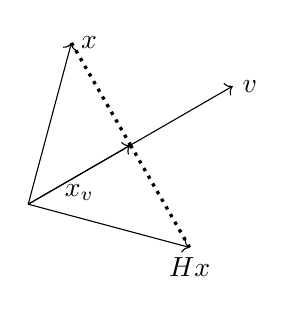
\begin{tikzpicture}[
        xscale = 1.5,
        yscale = 1.5,
        rotate = 30
        ]
        \draw[->] (0, 0) -- (1, 1) node[right] {$x$};
        \draw[->] (0, 0) -- (2, 0) node[right] {$v$};
        \draw[dotted, very thick] (1, 1) -- (1, 0);
        \draw[dotted, very thick] (1, 0) -- (1, -1);
        \draw[->] (0, 0) -- (1, 0) node[midway, below] {$x_v$};
        \draw[->] (0, 0) -- (1, -1) node[below] {$Hx$};
    \end{tikzpicture}
\end{figure}
The Household matrix acting on a vector $x$, $Hx$ is exactly the above case
since vector multiplication is associative we have
\begin{align}
    Hx &= x - \frac{2}{\langle v, v \rangle} vv^T x\\
       &= x - 2\frac{\langle v, x\rangle}{\langle v, v \rangle} v
\end{align}
The condition number of an orthogonal matrix $A$ in the $\|\cdot\|_2$ induced
norm is
\begin{align}
    K(A) =  \|A\|_2 \|A^{-1}\|_2 = 1,
\end{align}
because the orthogonal matrix preserves distance, i.e. $\|Ax\|_2 = \|x\|_2$
for all $x$. Also $A^{-1} =A^T$ is orthogonal as well
\begin{align}
    \|A\|_2 = \sup_{x\neq 0} \frac{\|Ax\|_2}{\|x\|_2} = \sup_{x \neq 0} \frac{\|x\|_2}{\|x\|_2} =
    1
\end{align}
%\printbibliography
\end{document}

